\newpage\handout
{Drill Problems: Week 2.5}
{\textsc{Scholastic Aptitude Test (SAT)}}
{\href{https://creativecommons.org/licenses/by-nc-sa/4.0/}{CC BY-NC-SA 4.0 license}}
{Author: \BookAuthor}{Release: \generatedOn}
{SAT: Drill Problems (2.5)}
% Copyright & Disclaimer
\begin{center}
  \begin{minipage}{0.85\textwidth}
    {\small\textbf{Purpose and Usage:}}\\[0.2cm]
    {\footnotesize
    This material has been developed for internal training and educational 
    purposes at Hans edu LLC. It is intended for use within our organization 
    and should not be distributed, sold, or used for commercial purposes 
    outside of our educational programs.}\\[0.5cm]
    
    {\small\textbf{For Our Community:}}\\[0.2cm]
    {\footnotesize
    Students and staff are welcome to use this material in their studies and 
    teaching at Hans edu LLC. While we encourage active engagement with the 
    content, please respect that this is proprietary material. Any 
    reproduction or distribution outside of our organization's educational 
    activities is not permitted.}\\[0.5cm]
    
    {\small\textbf{Content and Attribution:}}\\[0.2cm]
    {\footnotesize
    This material represents our adaptation of various established mathematics 
    textbooks, reorganized and enhanced for our teaching context. While we've 
    added our own pedagogical improvements, we maintain proper attribution to 
    original sources. This work is shared under the Creative Commons 
    Attribution-NonCommercial-ShareAlike (CC BY-NC-SA) license, allowing 
    internal use and adaptation while respecting the original creators' rights.
    % \small Key Permissions under CC BY-NC-SA 4.0:
    % \begin{itemize}
    %   \item credit the creator.
    %   \item no commercial use.
    %   \item new creations must carry the same license.
    %   \item copy and redistribute the material in any medium or format
    %   \item remix, transform, and build upon the material
    % \end{itemize}
    }\\[0.5cm]

    % Some content may be derived from sources under the CC0 1.0 Universal 
    % license, which allows for free use, modification, and distribution.}\\[0.5cm]
    {\small\textbf{Quality Assurance:}}\\[0.2cm]
    {\footnotesize
    We have carefully reviewed this material for accuracy and clarity. However, 
    as with any educational resource, we encourage critical engagement and 
    verification of concepts. If you notice any issues or have suggestions for 
    improvement, please bring them to our attention.}
  \end{minipage}
  
\includegraphics[width=0.45\textwidth]{images/CA_LastVersion.png}\\
  {\small © \the\year\ Hans edu LLC. All rights reserved.}\\[0.5cm]
  {\small Written by \BookAuthor}\\[1cm]
\end{center}

\newpage


\begin{enumerate}
  \item \textbf{Median Calculation} (10 points)\\
  What is the median of the seven data values shown?
  \[
  2,2,2,3,4,4,11
  \]
  \begin{enumerate}[label=(\Alph*)]
    \item 2
    \item 3
    \item 4
    \item 9
  \end{enumerate}
  \begin{subanswer}
    % your answer here
  \end{subanswer}

  \item \textbf{Box Plot Analysis} (10 points)\\
  The box plots summarize the masses, in kilograms, of two groups of gazelles.
  \begin{table}[h!]
  \centering
  \renewcommand{\arraystretch}{1.3}
  \setlength{\tabcolsep}{8pt}
  \begin{tabular}{cc}
  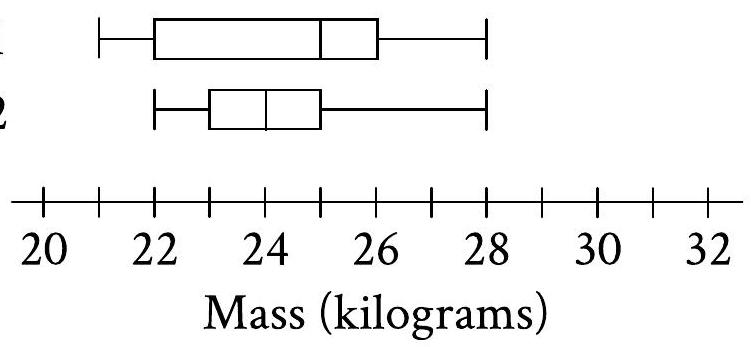
\includegraphics[width=0.4\textwidth]{images/2025_06_15_04f7426dc644de311e92g-02} &
  \end{tabular}
  \end{table}
  Based on the box plots, which of the following statements must be true?
  \begin{enumerate}[label=(\Alph*)]
    \item The mean mass of group 1 is greater than the mean mass of group 2.
    \item The mean mass of group 1 is less than the mean mass of group 2.
    \item The median mass of group 1 is greater than the median mass of group 2.
    \item The median mass of group 1 is less than the median mass of group 2.
  \end{enumerate}
  \begin{subanswer}
    % your answer here
  \end{subanswer}

  \newpage

  \item \textbf{Frequency Table Analysis} (10 points)\\
  Ages of 20 Students Enrolled in a College Class
  \begin{table}[h!]
  \centering
  \renewcommand{\arraystretch}{1.3}
  \setlength{\tabcolsep}{8pt}
  \caption*{\textbf{Ages of 20 Students Enrolled in a College Class}}
  \begin{tabular}{|c|c|}
  \hline
  \rowcolor[HTML]{E0E0E0}
  \textbf{Age} & \textbf{Frequency} \\
  \hline
  18 & 6 \\
  \hline
  19 & 5 \\
  \hline
  20 & 4 \\
  \hline
  21 & 2 \\
  \hline
  22 & 1 \\
  \hline
  23 & 1 \\
  \hline
  30 & 1 \\
  \hline
  \end{tabular}
  \end{table}
  The table above shows the distribution of ages of the 20 students enrolled in a college class. Which of the following gives the correct order of the mean, median, and mode of the ages?
  \begin{enumerate}[label=(\Alph*)]
    \item mode $<$ median $<$ mean
    \item mode $<$ mean $<$ median
    \item median $<$ mode $<$ mean
    \item mean $<$ mode $<$ median
  \end{enumerate}

  \begin{subanswer}
    % your answer here
  \end{subanswer}

  \item \textbf{Frequency Table Construction} (10 points)\\
  Which frequency table correctly represents the data listed?
  \[
  4,4,4,4,8,8,8,13,13
  \]
    \begin{table}[h!]
    \centering
    \renewcommand{\arraystretch}{1.3}
    \setlength{\tabcolsep}{8pt}
    \begin{tabular}{cccc}
    (A) &
    \begin{tabular}{|c|c|}
    \hline
    Number & Frequency \\
    \hline
    4 & 4 \\
    \hline
    8 & 3 \\
    \hline
    13 & 2 \\
    \hline
    \end{tabular}
    &
    (B) &
    \begin{tabular}{|c|c|}
    \hline
    Number & Frequency \\
    \hline
    4 & 4 \\
    \hline
    3 & 8 \\
    \hline
    2 & 13 \\
    \hline
    \end{tabular}
    \\
    (C) &
    \begin{tabular}{|c|c|}
    \hline
    Number & Frequency \\
    \hline
    4 & 16 \\
    \hline
    8 & 24 \\
    \hline
    13 & 26 \\
    \hline
    \end{tabular}
    &
    (D) &
    \begin{tabular}{|c|c|}
    \hline
    Number & Frequency \\
    \hline
    16 & 4 \\
    \hline
    24 & 8 \\
    \hline
    26 & 13 \\
    \hline
    \end{tabular}
    \end{tabular}
    \end{table}
  \begin{subanswer}
    % your answer here
  \end{subanswer}

  \newpage

  \item \textbf{Maximum Data Value} (10 points)\\
  \begin{table}[h!]
  \centering
  \renewcommand{\arraystretch}{1.3}
  \setlength{\tabcolsep}{8pt}
  \caption*{\textbf{Frequency Table}}
  \begin{tabular}{|c|c|}
  \hline
  \rowcolor[HTML]{E0E0E0}
  \textbf{Data value} & \textbf{Frequency} \\
  \hline
  6 & 3 \\
  \hline
  7 & 3 \\
  \hline
  8 & 8 \\
  \hline
  9 & 8 \\
  \hline
  10 & 9 \\
  \hline
  11 & 11 \\
  \hline
  12 & 9 \\
  \hline
  13 & 0 \\
  \hline
  14 & 6 \\
  \hline
  \end{tabular}
  \end{table}
  The frequency table summarizes the 57 data values in a data set. What is the maximum data value in the data set?
  \begin{subanswer}
    % your answer here
  \end{subanswer}

  \item \textbf{Mean Equality} (10 points)\\
  Data set $A$ and data set $B$ each contain 5 numbers.
  \[
  \text{Data set A: }72,73,73,76,76
  \]
  \[
  \text{Data set B: }61, 64, 74, 85, x
  \]
  If the mean of data set $A$ is equal to the mean of data set $B$, what is the value of $x$?
  \begin{enumerate}[label=(\Alph*)]
    \item 77
    \item 85
    \item 86
    \item 95
  \end{enumerate}
  \begin{subanswer}
    % your answer here
  \end{subanswer}

  \item \textbf{Statistical Calculations} (10 points)\\
  For a school fund-raiser, 10 students sold a total of 90 boxes of cookies. Which of the following can be calculated from this information?
  \begin{enumerate}[label=(\Alph*)]
    \item The average number of boxes sold per student
    \item The median number of boxes sold per student
    \item The greatest number of boxes sold by one student
    \item The least number of boxes sold by one student
  \end{enumerate}
  \begin{subanswer}
    % your answer here
  \end{subanswer}

  \item \textbf{Standard Deviation Comparison} (10 points)\\
  The results of two independent surveys are shown in the table below.
  \begin{table}[h!]
  \centering
  \renewcommand{\arraystretch}{1.3}
  \setlength{\tabcolsep}{8pt}
  \caption*{\textbf{Men's Height Survey Results}}
  \begin{tabular}{|c|c|c|c|}
  \hline
  \rowcolor[HTML]{E0E0E0}
  \textbf{Group} & \textbf{Sample Size} & \textbf{Mean (cm)} & \textbf{Std. Dev. (cm)} \\
  \hline
  A & 2,500 & 186 & 12.5 \\
  B & 2,500 & 186 & 19.1 \\
  \hline
  \end{tabular}
  \end{table}
  Which statement is true based on the table?
  \begin{enumerate}[label=(\Alph*)]
    \item The Group A data set was identical to the Group B data set.
    \item Group B contained the tallest participant.
    \item The heights of the men in Group B had a larger spread than the heights of the men in Group A.
    \item The median height of Group B is larger than the median height of Group A.
  \end{enumerate}
  \begin{subanswer}
    % your answer here
  \end{subanswer}

  \item \textbf{Mean and Median Equality} (10 points)\\
  The mean and the median of the five numbers above are equal.
  \[
  15,14,18,17, x
  \]
  Which of the following is NOT a possible value of $x$?
  \begin{enumerate}[label=(\Alph*)]
    \item 6
    \item 11
    \item 16
    \item 21
  \end{enumerate}
  \begin{subanswer}
    % your answer here
  \end{subanswer}

  \item \textbf{Missing Data Value} (10 points)\\
  Data set A consists of 10 positive integers less than 60. The list shown gives 9 of the integers from data set A.
  \[
  43,45,44,43,38,39,40,46,40
  \]
  The mean of these 9 integers is 42. If the mean of data set A is an integer that is greater than 42, what is the value of the largest integer from data set A?
  \begin{subanswer}
    % your answer here
  \end{subanswer}


  \newpage

  \item \textbf{Scatterplot Analysis} (10 points)\\
  Distance and Density of Planetoids in the Inner Solar System
  \insertimage{0.40}{images/2025_06_15_c6d1fe032100fbb48447g-01}{reference attached}
  The scatterplot above shows the densities of 7 planetoids, in grams per cubic centimeter, with respect to their average distances from the Sun in astronomical units (AU). The line of best fit is also shown. An astronomer has discovered a new planetoid about 1.2 AU from the Sun. According to the line of best fit, which of the following best approximates the density of the planetoid, in grams per cubic centimeter?
  \begin{enumerate}[label=(\Alph*)]
    \item 3.6
    \item 4.1
    \item 4.6
    \item 5.5
  \end{enumerate}
  \begin{subanswer}
    % your answer here
  \end{subanswer}

  \item \textbf{Investment Growth Model} (10 points)\\
  Each year, the value of an investment increases by $0.49\%$ of its value the previous year. Which of the following functions best models how the value of the investment changes over time?
  \begin{enumerate}[label=(\Alph*)]
    \item Decreasing exponential
    \item Decreasing linear
    \item Increasing exponential
    \item Increasing linear
  \end{enumerate}
  \begin{subanswer}
    % your answer here
  \end{subanswer}

  \newpage

  \item \textbf{Line of Best Fit Slope} (10 points)\\
  The scatterplot shows the relationship between $x$ and $y$. A line of best fit is also shown.
  \insertimage{0.40}{images/2025_06_15_c6d1fe032100fbb48447g-03}{reference attached}
  Which of the following is closest to the slope of the line of best fit shown?
  \begin{enumerate}[label=(\Alph*)]
    \item -2.27
    \item -0.44
    \item 0.44
    \item 2.27
  \end{enumerate}
  \begin{subanswer}
    % your answer here
  \end{subanswer}

  \newpage

  \item \textbf{Protein and Fat Correlation} (10 points)\\
  \insertimage{0.40}{images/2025_06_15_c6d1fe032100fbb48447g-04}{reference attached}
  The scatterplot above shows the numbers of grams of both total protein and total fat for eight sandwiches on a restaurant menu. The line of best fit for the data is also shown. According to the line of best fit, which of the following is closest to the predicted increase in total fat, in grams, for every increase of 1 gram in total protein?
  \begin{enumerate}[label=(\Alph*)]
    \item 2.5
    \item 2.0
    \item 1.5
    \item 1.0
  \end{enumerate}
  \begin{subanswer}
    % your answer here
  \end{subanswer}


  \newpage

  \item \textbf{Linear Model Selection} (10 points)\\
  The scatterplot shows the relationship between two variables, $x$ and $y$.
  \insertimage{0.30}{images/cus12.png}{reference attached}
  Which of the following equations is the most appropriate linear model for the data shown?
  \begin{enumerate}[label=(\Alph*)]
    \item $y=0.9+9.4 x$
    \item $y=0.9-9.4 x$
    \item $y=9.4+0.9 x$
    \item $y=9.4-0.9 x$
  \end{enumerate}
  \begin{subanswer}
    % your answer here
  \end{subanswer}

  \item \textbf{Investment Comparison} (10 points)\\
  \begin{table}[h!]
  \centering
  \renewcommand{\arraystretch}{1.3}
  \setlength{\tabcolsep}{8pt}
  \caption*{\textbf{Investment Comparison}}
  \begin{tabular}{|c|c|c|}
  \hline
  \rowcolor[HTML]{E0E0E0}
   & \textbf{Amount invested} & \textbf{Balance increase} \\
  \hline
  Account A & $\$ 500$ & $6\%$ annual interest \\
  \hline
  Account B & $\$ 1,000$ & $\$ 25$ per year \\
  \hline
  \end{tabular}
  \end{table}
  Two investments were made as shown in the table above. The interest in Account A is compounded once per year. Which of the following is true about the investments?
  \begin{enumerate}[label=(\Alph*)]
    \item Account A always earns more money per year than Account B.
    \item Account A always earns less money per year than Account B.
    \item Account A earns more money per year than Account B at first but eventually earns less money per year.
    \item Account A earns less money per year than Account B at first but eventually earns more money per year.
  \end{enumerate}
  \begin{subanswer}
    % your answer here
  \end{subanswer}

  \item \textbf{Function Classification} (10 points)\\
  For $x>0$, the function $f$ is defined as follows:
  \[
  f(x) \text{ equals } 201\% \text{ of } x
  \]
  Which of the following could describe this function?
  \begin{enumerate}[label=(\Alph*)]
    \item Decreasing exponential
    \item Decreasing linear
    \item Increasing exponential
    \item Increasing linear
  \end{enumerate}
  \begin{subanswer}
    % your answer here
  \end{subanswer}

  \item \textbf{Prediction from Line of Best Fit} (10 points)\\
  The scatterplot shows the relationship between two variables, $x$ and $y$. A line of best fit for the data is also shown.
  \insertimage{0.40}{images/2025_06_15_c6d1fe032100fbb48447g-08}{reference attached}
  At $x=32$, which of the following is closest to the $y$-value predicted by the line of best fit?
  \begin{enumerate}[label=(\Alph*)]
    \item 0.4
    \item 1.5
    \item 2.4
    \item 3.3
  \end{enumerate}
  \begin{subanswer}
    % your answer here
  \end{subanswer}

  \newpage

  \item \textbf{House Price Model} (10 points)\\
  \insertimage{0.40}{images/2025_06_15_c6d1fe032100fbb48447g-09}{reference attached}
  The scatterplot above shows the size $x$ and the sale price $y$ of 25 houses for sale in Town H. Which of the following could be an equation for a line of best fit for the data?
  \begin{enumerate}[label=(\Alph*)]
    \item $y=200 x+100$
    \item $y=100 x+100$
    \item $y=50 x+100$
    \item $y=100 x$
  \end{enumerate}
  \begin{subanswer}
    % your answer here
  \end{subanswer}

  \newpage

  \item \textbf{Elevation and Temperature Association} (10 points)\\
  \insertimage{0.40}{images/2025_06_15_c6d1fe032100fbb48447g-10}{reference attached}
  The scatterplot above shows the high temperature on a certain day and the elevation of 8 different locations in the Lake Tahoe Basin. A line of best fit for the data is also shown. Which of the following statements best describes the association between the elevation and the temperature of locations in the Lake Tahoe Basin?
  \begin{enumerate}[label=(\Alph*)]
    \item As the elevation increases, the temperature tends to increase.
    \item As the elevation increases, the temperature tends to decrease.
    \item As the elevation decreases, the temperature tends to decrease.
    \item There is no association between the elevation and the temperature.
  \end{enumerate}
  \begin{subanswer}
    % your answer here
  \end{subanswer}
  \item \textbf{Printer Rate Conversion} (10 points)\\
  A printer produces posters at a constant rate of 42 posters per minute. At what rate, in posters per hour, does the printer produce the posters?
  \begin{subanswer}
    % your answer here
  \end{subanswer}

  \newpage

  \item \textbf{Speed Conversion} (10 points)\\
  The International Space Station orbits Earth at an average speed of 4.76 miles per second. What is the space station's average speed in miles per hour?
  \begin{enumerate}[label=(\Alph*)]
    \item 285.6
    \item 571.2
    \item 856.8
    \item $17136.0$
  \end{enumerate}
  \begin{subanswer}
    % your answer here
  \end{subanswer}

  \item \textbf{Lightning Distance Calculation} (10 points)\\
  For a person $m$ miles from a flash of lightning, the length of the time interval from the moment the person sees the lightning to the moment the person hears the thunder is $k$ seconds. The ratio of $m$ to $k$ can be estimated to be 1 to 5. According to this estimate, the person is how many miles from a flash of lightning if the time interval is 25 seconds?
  \begin{enumerate}[label=(\Alph*)]
    \item 10
    \item 9
    \item 6
    \item 5
  \end{enumerate}
  \begin{subanswer}
    % your answer here
  \end{subanswer}

  \item \textbf{Population Increase Calculation} (10 points)\\
  The population density of Iceland, in people per square kilometer of land area, increased from 2.5 in 1990 to 3.3 in 2014. During this time period, the land area of Iceland was 100,250 square kilometers. By how many people did Iceland's population increase from 1990 to 2014?
  \begin{enumerate}[label=(\Alph*)]
    \item 330,825
    \item 132,330
    \item 125,312
    \item 80,200
  \end{enumerate}
  \begin{subanswer}
    % your answer here
  \end{subanswer}

  \item \textbf{Orange Purchase Calculation} (10 points)\\
  A customer spent $\$ 27$ to purchase oranges at $\$ 3$ per pound. How many pounds of oranges did the customer purchase?
  \begin{subanswer}
    % your answer here
  \end{subanswer}

  \item \textbf{Butterfly Migration Rate} (10 points)\\
  A group of monarch butterflies migrated from Chicago, Illinois, to Michoacán, Mexico, flying a total of 2,100 miles. It took a single butterfly in the group 120 days to travel this route one way. On average, how many miles did the butterfly travel per day?
  \begin{enumerate}[label=(\Alph*)]
    \item 0.057
    \item 0.729
    \item 17.5
    \item 24
  \end{enumerate}
  \begin{subanswer}
    % your answer here
  \end{subanswer}

  \item \textbf{Proportional Relationship} (10 points)\\
  If $\frac{x}{y}=4$ and $\frac{24 x}{n y}=4$, what is the value of $n$?
  \begin{subanswer}
    % your answer here
  \end{subanswer}

  \item \textbf{Ratio Problem} (10 points)\\
  In a box of pens, the ratio of black pens to red pens is 8 to 1. There are 40 black pens in the box. How many red pens are in the box?
  \begin{enumerate}[label=(\Alph*)]
    \item 5
    \item 8
    \item 40
    \item 320
  \end{enumerate}
  \begin{subanswer}
    % your answer here
  \end{subanswer}

  \item \textbf{Density and Price Calculation} (10 points)\\
  Pure beeswax has a density of 0.555 ounce per cubic inch. An online company sells pure beeswax at a price of $\$ 8.00$ per ounce. What is the selling price, in dollars per cubic inch, for pure beeswax purchased from this company?
  \begin{subanswer}
    % your answer here
  \end{subanswer}

  \newpage

  \item \textbf{Area Calculation} (10 points)\\
  The population density of Worthington is 290 people per square mile. Worthington has a population of 92,800 people. What is the area, in square miles, of Worthington?
  \begin{enumerate}[label=(\Alph*)]
    \item 102,400
    \item 93,090
    \item 320
    \item 32
  \end{enumerate}
  \begin{subanswer}
    % your answer here
  \end{subanswer}

  \item \textbf{Percentage Expression} (10 points)\\
  Jennifer bought a box of Crunchy Grain cereal. The nutrition facts on the box state that a serving size of the cereal is $\frac{3}{4}$ cup and provides 210 calories, 50 of which are calories from fat. In addition, each serving of the cereal provides 180 milligrams of potassium, which is $5\%$ of the daily allowance for adults. If $p$ percent of an adult's daily allowance of potassium is provided by $x$ servings of Crunchy Grain cereal per day, which of the following expresses $p$ in terms of $x$?
  \begin{enumerate}[label=(\Alph*)]
    \item $p=0.5 x$
    \item $p=5 x$
    \item $p=(0.05)^{x}$
    \item $p=(1.05)^{x}$
  \end{enumerate}
  \begin{subanswer}
    % your answer here
  \end{subanswer}

  \item \textbf{Committee Composition} (10 points)\\
  A school district is forming a committee to discuss plans for the construction of a new high school. Of those invited to join the committee, 15\% are parents of students, 45\% are teachers from the current high school, 25\% are school and district administrators, and the remaining 6 individuals are students. How many more teachers were invited to join the committee than school and district administrators?
  \begin{subanswer}
    % your answer here
  \end{subanswer}

  \newpage

  \item \textbf{Percent Increase Calculation} (10 points)\\
  A table of the US minimum wage for 6 different years is shown below.
  \begin{table}[h!]
  \centering
  \renewcommand{\arraystretch}{1.3}
  \setlength{\tabcolsep}{8pt}
  \caption*{\textbf{US Minimum Wage by Year}}
  \begin{tabular}{|c|c|}
  \hline
  \rowcolor[HTML]{E0E0E0}
  \textbf{Year} & \textbf{US Minimum Wage (dollars per hour)} \\
  \hline
  1960 & \$1.00 \\
  \hline
  1970 & \$1.60 \\
  \hline
  1980 & \$3.10 \\
  \hline
  1990 & \$3.80 \\
  \hline
  2000 & \$5.15 \\
  \hline
  2010 & \$7.25 \\
  \hline
  \end{tabular}
  \end{table}
  What was the percent increase of the minimum wage from 1960 to 1970?
  \begin{enumerate}[label=(\Alph*)]
    \item $30\%$
    \item $60\%$
    \item $62.5\%$
    \item $120\%$
  \end{enumerate}
  \begin{subanswer}
    % your answer here
  \end{subanswer}

  \item \textbf{Subscription Growth} (10 points)\\
  \begin{table}[h!]
  \centering
  \renewcommand{\arraystretch}{1.3}
  \setlength{\tabcolsep}{8pt}
  \caption*{\textbf{Subscription Sales}}
  \begin{tabular}{|c|c|}
  \hline
  \rowcolor[HTML]{E0E0E0}
  \textbf{Year} & \textbf{Subscriptions sold} \\
  \hline
  2012 & 5,600 \\
  \hline
  2013 & 5,880 \\
  \hline
  \end{tabular}
  \end{table}
  The manager of an online news service received the report above on the number of subscriptions sold by the service. The manager estimated that the percent increase from 2012 to 2013 would be double the percent increase from 2013 to 2014. How many subscriptions did the manager expect would be sold in 2014?
  \begin{enumerate}[label=(\Alph*)]
    \item 6,020
    \item 6,027
    \item 6,440
    \item 6,468
  \end{enumerate}
  \begin{subanswer}
    % your answer here
  \end{subanswer}

  \newpage

  \item \textbf{Snowfall Decrease} (10 points)\\
  \insertimage{0.40}{images/2025_06_15_685e39be57606e31d5a9g-05}{reference attached}
  The line graph shows the total amount of snow, in inches, recorded each year in Washington, DC, from 2003 to 2015. If $p\%$ is the percent decrease in the annual snowfall from 2003 to 2007, what is the value of $p$?
  \begin{subanswer}
    % your answer here
  \end{subanswer}

  \item \textbf{Percentage Calculation} (10 points)\\
  What percentage of 300 is 75?
  \begin{enumerate}[label=(\Alph*)]
    \item $25\%$
    \item $50\%$
    \item $75\%$
    \item $225\%$
  \end{enumerate}
  \begin{subanswer}
    % your answer here
  \end{subanswer}

  \item \textbf{Sales Tax Calculation} (10 points)\\
  The cost of a certain shirt is \$20 before a 5\% sales tax is added. What is the total cost, including sales tax, to purchase the shirt?
  \begin{enumerate}[label=(\Alph*)]
    \item $\$ 20.05$
    \item $\$ 20.50$
    \item $\$ 21.00$
    \item $\$ 25.00$
  \end{enumerate}
  \begin{subanswer}
    % your answer here
  \end{subanswer}

  \item \textbf{Voting Analysis} (10 points)\\
  For the finale of a TV show, viewers could use either social media or a text message to vote for their favorite of two contestants. The contestant receiving more than $50\%$ of the vote won. An estimated $10\%$ of the viewers voted, and $30\%$ of the votes were cast on social media. Contestant 2 earned $70\%$ of the votes cast using social media and $40\%$ of the votes cast using a text message. Based on this information, which of the following is an accurate conclusion?
  \begin{enumerate}[label=(\Alph*)]
    \item If all viewers had voted, Contestant 2 would have won.
    \item Viewers voting by social media were likely to be younger than viewers voting by text message.
    \item If all viewers who voted had voted by social media instead of by text message, Contestant 2 would have won.
    \item Viewers voting by social media were more likely to prefer Contestant 2 than were viewers voting by text message.
  \end{enumerate}
  \begin{subanswer}
    % your answer here
  \end{subanswer}

  \item \textbf{Return Rate Calculation} (10 points)\\
  During the first month of sales, a company sold 1,300,000 units of a certain type of smartphone. During the same month, $15\%$ of the units sold were returned. If sales and the return rate remain the same for each of the next 5 months, about how many units of this smartphone will be returned to the company during this 6-month period?
  \begin{enumerate}[label=(\Alph*)]
    \item 195,000
    \item 975,000
    \item $1,170,000$
    \item $6,630,000$
  \end{enumerate}
  \begin{subanswer}
    % your answer here
  \end{subanswer}

  \item \textbf{Enrollment Increase} (10 points)\\
  Last year, 200 students enrolled in an interior design program. This year, the number of students enrolled is $147\%$ of last year's number. How many students are enrolled in the interior design program this year?
  \begin{enumerate}[label=(\Alph*)]
    \item 247
    \item 294
    \item 347
    \item 394
  \end{enumerate}
  \begin{subanswer}
    % your answer here
  \end{subanswer}

  \newpage

  \item \textbf{Cell Phone Study Analysis} (10 points)\\
  \begin{table}[h!]
  \centering
  \renewcommand{\arraystretch}{1.3}
  \setlength{\tabcolsep}{8pt}
  \caption*{\textbf{Cell Phone Use Study}}
  \begin{tabular}{|l|l|l|l|}
  \hline
  \rowcolor[HTML]{E0E0E0}
  \textbf{Texting behavior} & \textbf{Talks on cell phone daily} & \textbf{Does not talk on cell phone daily} & \textbf{Total} \\
  \hline
  Light & 110 & 146 & 256 \\
  \hline
  Medium & 139 & 164 & 303 \\
  \hline
  Heavy & 166 & 74 & 240 \\
  \hline
  Total & 415 & 384 & 799 \\
  \hline
  \end{tabular}
  \end{table}
  In a study of cell phone use, 799 randomly selected US teens were asked how often they talked on a cell phone and about their texting behavior. The data are summarized in the table above. Based on the data from the study, an estimate of the percent of US teens who are heavy texters is $30\%$ and the associated margin of error is $3\%$. Which of the following is a correct statement based on the given margin of error?
  \begin{enumerate}[label=(\Alph*)]
    \item Approximately $3\%$ of the teens in the study who are classified as heavy texters are not really heavy texters.
    \item It is not possible that the percent of all US teens who are heavy texters is less than $27\%$.
    \item The percent of all US teens who are heavy texters is $33\%$.
    \item It is doubtful that the percent of all US teens who are heavy texters is $35\%$.
  \end{enumerate}
  \begin{subanswer}
    % your answer here
  \end{subanswer}

  \item \textbf{Survey Estimation} (10 points)\\
  There are 55 students in Spanish club. A sample of the Spanish club students was selected at random and asked whether they intend to enroll in a new study program. Of those surveyed, $20\%$ responded that they intend to enroll in the study program. Based on this survey, which of the following is the best estimate of the total number of Spanish club students who intend to enroll in the study program?
  \begin{enumerate}[label=(\Alph*)]
    \item 11
    \item 20
    \item 44
    \item 55
  \end{enumerate}
  \begin{subanswer}
    % your answer here
  \end{subanswer}

  \newpage

  \item \textbf{Nuclear Energy Survey} (10 points)\\
    \begin{table}[h!]
    \centering
    \renewcommand{\arraystretch}{1.3}
    \setlength{\tabcolsep}{8pt}
    \caption*{\textbf{Views on Nuclear Energy}}
    \begin{tabular}{|l|c|}
    \hline
    \rowcolor[HTML]{E0E0E0}
    \textbf{Response} & \textbf{Frequency} \\
    \hline
    Strongly favor    & 56  \\
    Somewhat favor    & 214 \\
    Somewhat oppose   & 104 \\
    Strongly oppose   & 37  \\
    \hline
    \end{tabular}
    \end{table}
  A researcher interviewed 411 randomly selected US residents and asked about their views on the use of nuclear energy. The table above summarizes the responses of the interviewees. If the population of the United States was 300 million when the survey was given, based on the sample data for the 411 US residents, what is the best estimate, in millions, of the difference between the number of US residents who somewhat favor or strongly favor the use of nuclear energy and the number of those who somewhat oppose or strongly oppose it? (Round your answer to the nearest whole number.)
  \begin{subanswer}
    % your answer here
  \end{subanswer}

  \item \textbf{Contest Probability} (10 points)\\
  \begin{table}[h!]
  \centering
  \renewcommand{\arraystretch}{1.3}
  \setlength{\tabcolsep}{8pt}
  \caption*{\textbf{Number of Contestants by Score and Day}}
  \begin{tabular}{|l|l|l|l|l|l|l|l|}
  \hline
  \rowcolor[HTML]{E0E0E0}
   & \textbf{5 out of 5} & \textbf{4 out of 5} & \textbf{3 out of 5} & \textbf{2 out of 5} & \textbf{1 out of 5} & \textbf{0 out of 5} & \textbf{Total} \\
  \hline
  Day 1 & 2 & 3 & 4 & 6 & 2 & 3 & 20 \\
  \hline
  Day 2 & 2 & 3 & 5 & 5 & 4 & 1 & 20 \\
  \hline
  Day 3 & 3 & 3 & 4 & 5 & 3 & 2 & 20 \\
  \hline
  Total & 7 & 9 & 13 & 16 & 9 & 6 & 60 \\
  \hline
  \end{tabular}
  \end{table}
  The same 20 contestants, on each of 3 days, answered 5 questions in order to win a prize. Each contestant received 1 point for each correct answer. The number of contestants receiving a given score on each day is shown in the table above. No contestant received the same score on two different days. If a contestant is selected at random, what is the probability that the selected contestant received a score of 5 on Day 2 or Day 3, given that the contestant received a score of 5 on one of the three days?
  \begin{subanswer}
    % your answer here
  \end{subanswer}

  \newpage

  \item \textbf{Dice Probability} (10 points)\\
  Each face of a fair 14-sided die is labeled with a number from 1 through 14, with a different number appearing on each face. If the die is rolled one time, what is the probability of rolling a 2?
  \begin{enumerate}[label=(\Alph*)]
    \item $\frac{1}{14}$
    \item $\frac{2}{14}$
    \item $\frac{12}{14}$
    \item $\frac{13}{14}$
  \end{enumerate}
  \begin{subanswer}
    % your answer here
  \end{subanswer}

  \item \textbf{Car Selection Probability} (10 points)\\
  \begin{table}[h!]
  \centering
  \renewcommand{\arraystretch}{1.3}
  \setlength{\tabcolsep}{8pt}
  \caption*{\textbf{Prices of 14 Different Cars}}
  \begin{tabular}{|c|c|c|c|}
  \hline
  \rowcolor[HTML]{E0E0E0}
  \textbf{Type of car} & \begin{tabular}{c}
  \textbf{Priced at no more} \\
  \textbf{than \$25,000} \\
  \end{tabular} & \begin{tabular}{c}
  \textbf{Priced greater} \\
  \textbf{than \$25,000} \\
  \end{tabular} & \textbf{Total} \\
  \hline
  Nonhybrid & 5 & 3 & 8 \\
  \hline
  Hybrid & 2 & 4 & 6 \\
  \hline
  Total & 7 & 7 & 14 \\
  \hline
  \end{tabular}
  \end{table}
  The table above shows information about 14 cars listed for sale on an auto dealership's website. If one of the cars listed for sale is selected at random, what is the probability that the car selected will be a hybrid car priced at no more than $\$ 25,000$?
  \begin{enumerate}[label=(\Alph*)]
    \item $\frac{1}{7}$
    \item $\frac{2}{7}$
    \item $\frac{1}{3}$
    \item $\frac{4}{7}$
  \end{enumerate}
  \begin{subanswer}
    % your answer here
  \end{subanswer}

  \newpage

  \item \textbf{Marble Probability} (10 points)\\
  Colors of Marbles in a Bag
  \begin{table}[h!]
  \centering
  \renewcommand{\arraystretch}{1.3}
  \setlength{\tabcolsep}{8pt}
  \caption*{\textbf{Colors of Marbles in a Bag}}
  \begin{tabular}{|c|c|}
  \hline
  \rowcolor[HTML]{E0E0E0}
  \textbf{Color} & \textbf{Number} \\
  \hline
  Red & 8 \\
  \hline
  Blue & 10 \\
  \hline
  Green & 22 \\
  \hline
  Total & 40 \\
  \hline
  \end{tabular}
  \end{table}
  The table shows the number of different colors of marbles in a bag. If a marble is chosen at random from the bag, what is the probability that the marble will be blue?
  \begin{enumerate}[label=(\Alph*)]
    \item $\frac{30}{40}$
    \item $\frac{22}{40}$
    \item $\frac{18}{40}$
    \item $\frac{10}{40}$
  \end{enumerate}
  \begin{subanswer}
    % your answer here
  \end{subanswer}

  \item \textbf{Gas Station Probability} (10 points)\\
  Customer Purchases at a Gas Station
  \begin{table}[h!]
  \centering
  \renewcommand{\arraystretch}{1.3}
  \setlength{\tabcolsep}{8pt}
  \caption*{\textbf{Customer Purchases at a Gas Station}}
  \begin{tabular}{|c|c|c|c|}
  \hline
  \rowcolor[HTML]{E0E0E0}
   & \textbf{Beverage purchased} & \textbf{Beverage not purchased} & \textbf{Total} \\
  \hline
  Gasoline purchased & 60 & 25 & 85 \\
  \hline
  Gasoline not purchased & 35 & 15 & 50 \\
  \hline
  Total & 90 & 40 & 135 \\
  \hline
  \end{tabular}
  \end{table}
  On Tuesday, a local gas station had 135 customers. The table above summarizes whether or not the customers on Tuesday purchased gasoline, a beverage, both, or neither. Based on the data in the table, what is the probability that a gas station customer selected at random on that day did not purchase gasoline?
  \begin{enumerate}[label=(\Alph*)]
    \item $\frac{15}{50}$
    \item $\frac{15}{40}$
    \item $\frac{35}{50}$
    \item $\frac{50}{135}$
  \end{enumerate}
  \begin{subanswer}
    % your answer here
  \end{subanswer}

  \item \textbf{Survey Population} (10 points)\\
  A sample of 40 fourth-grade students was selected at random from a certain school. The 40 students completed a survey about the morning announcements, and 32 thought the announcements were helpful. Which of the following is the largest population to which the results of the survey can be applied?
  \begin{enumerate}[label=(\Alph*)]
    \item The 40 students who were surveyed
    \item All fourth-grade students at the school
    \item All students at the school
    \item All fourth-grade students in the county in which the school is located
  \end{enumerate}
  \begin{subanswer}
    % your answer here
  \end{subanswer}

  \item \textbf{Satisfaction Survey} (10 points)\\
  Residents of a town were surveyed to determine whether they are satisfied with the concession stand at the local park. A random sample of 200 residents was selected. All 200 responded, and $87\%$ said they are satisfied. Based on this information, which of the following statements must be true?
  \begin{enumerate}[label=(\Roman*)]
    \item Of all the town residents, $87\%$ would say they are satisfied with the concession stand at the local park.
    \item If another random sample of 200 residents were surveyed, $87\%$ would say they are satisfied.
  \end{enumerate}
  \begin{enumerate}[label=(\Alph*)]
    \item Neither
    \item I only
    \item II only
    \item I and II
  \end{enumerate}
  \begin{subanswer}
    % your answer here
  \end{subanswer}
\end{enumerate}




